\chapter{Let's Get Started}
\label{ch:lgstarted}
% ##################################################################################################################
\hfill \textbf{Author:} Andreas Horni, ... 

\begin{center} 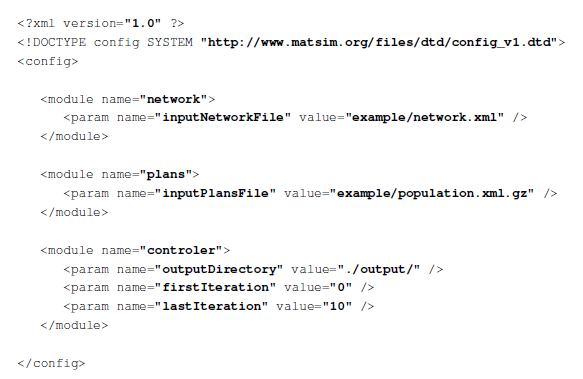
\includegraphics[width=0.7\textwidth, angle=0]{using/figures/config.png} \end{center}

% ##################################################################################################################
This chapter explains how to set up and run MATSim and it describes the requirements of building a basic scenario. As this book tries to be as stable and timeless as possible, the MATSim user guide \citep[][]{MATSim_Userguide_2014} needs to be consulted in addition to this chapter for doing an actual installation; frequently changing and detailed information such as download paths or version-dependent configurations are omitted here and left to the user guide. 

Getting the source code into different computing environments and extending MATSim through the API is described in the second part of the book in Chapter~\ref{ch:extensionpoints}.

% ##################################################################################################################
\section{Running MATSim}
\label{sec:runningmatsim}
% ================================================================================================
\subsection{Setting Up MATSim}
To run MATSim you have to install the Java Platform Standard Edition (SE) that complies with the MATSim version to be run. At the time of writing this book, this is JAVA SE 7.

Furthermore you need the official MATSim release, which comes as a zip file (usually named with the version number \lstinline|matsim-yy.yy.yy.zip|) including everything that is required to run it. It can be downloaded following the links on the MATSim web page. Unzip it and continue with Section~\ref{sec:runexample}.

If you prefer to use the more up to date nightly builds, you need to manually download the matsim jar file (usually named with the revision number \lstinline|MATSim_ryyyy.jar|) and the required external libraries (\lstinline|MATSim_libs.zip|). Unzipping this collection of 3rd-party libraries, you should then get a directory \lstinline|libs| with several jar-files inside. If the directory \lstinline|libs| is in the same directory as the MATSim jar-file, the libraries are found automatically and must not be added to the \lstinline|classpath| manually.

% ================================================================================================
\subsection{Running MATSim}
\label{sec:runexample}
MATSim does not provide a graphical user interface, thus, you need to be able to handle and access a command line tool. In Linux or Mac OS X, this is typically a Terminal application, and in Windows, the Power Shell or Command Prompt.

On the command prompt type the following command as one line, but substitute the correct paths: 

\lstinline|java -Xmx512m -cp /path/to/matsim.jar org.matsim.run.Controler /path/to/config.xml|

As an example, on Linux this could look like: \\
\lstinline|java -Xmx512m -cp /home/username/matsim/matsim.jar org.matsim.run.Controler /home/user/matsim/input/config.xml|

On Mac OS X, it could look like this: \\
\lstinline|java -Xmx512m -cp /Users/username/matsim/matsim.jar org.matsim.run.Controler /Users/user/matsim/input/config.xml|

On Windows, an example command could be: \\
\lstinline|java -Xmx512m -cp C:\MATSim\matsim.jar org.matsim.run.Controler C:\MATSim\input\config.xml|

Such a command exists of multiple parts:
\begin{itemize}
\item \lstinline|java| tells the system that you want to run Java.
\item \lstinline|-Xmx512m| tells Java that it should use up to 512 MB of memory. This is typically enough to run the small examples. For larger scenarios, you might need more memory, e.g., \lstinline|-Xmx3g| would allow Java to use up to 3 GB of memory.
\item \lstinline|-cp /path/to/matsim.jar| tells Java where to find the MATSim code.
\item \lstinline|org.matsim.run.Controler| specifies which class (think of an ``entry point'') should be run. In most cases, the default MATSim Controler is the class you'll need to run simulations.
\item \lstinline|/path/to/config.xml| tells MATSim which config file is to be used.
\end{itemize}

% ================================================================================================
\subsection{Configuring MATSim}
Configuring MATSim is (at this stage) only done via the configuration file, often just referred to as \lstinline|config file| or as \lstinline|config.xml|. It builds the connection between the user and MATSim. It contains a list of settings which influence how the simulation behaves. In the second part of the book we will learn how MATSim can be configured and extended by programming against its API.

All configuration parameters are simple pairs of a parameter \lstinline|name| and a parameter \lstinline|value|. The parameters are grouped into logical groups. For example, there is a group with settings related to the Controler like the number of iterations, or there is another group with settings related to the simulation, e.g. the end time of the simulation. As shown in Chapter~\ref{ch:modules}, a whole bunch of MATSim modules can be added to MATSim and configured by specifying the respective section of the configuration file.

A minimal configuration file is shown below, specifying the minimal information, MATSim needs about demand and supply and about the run configuration. In the example, supply is given by the network, demand is given in the plans file (typical input data produced is described in Section \ref{sec:inputdata}), and the controler is run for 10 iterations with the given output directory (typical output data produced is described in Section \ref{sec:outputdata}).

\begin{lstlisting}
<?xml version="1.0" ?> 
<!DOCTYPE config SYSTEM "http://www.matsim.org/files/dtd/config_v1.dtd"> 
<config> 
 
   <module name="network"> 
      <param name="inputNetworkFile" value="example/network.xml" /> 
   </module> 
 
   <module name="plans"> 
      <param name="inputPlansFile" value="example/population.xml.gz" /> 
   </module> 
 
   <module name="controler"> 
      <param name="outputDirectory" value="./output/" /> 
      <param name="firstIteration" value="0" /> 
      <param name="lastIteration" value="10" /> 
   </module> 
 
</config>
\end{lstlisting}

The list of available parameters and valid parameter values may vary from release to release. Although we try to keep this stable, due to changes in the software, most notably by new features, settings may change. To get a list of all available settings currently available, run the following command: \lstinline|java -cp matsim.jar org.matsim.run.CreateFullConfig fullConfig.xml|.

This command will create a new config file \lstinline|fullConfig.xml|, which contains the full list of available parameters along with their default values. This makes it easy to see what settings are available. To use and modify certain settings, the lines with the corresponding parameters can be copied to the config file specific for the scenario to be simulated and the parameter values be modified in that file. 

% ##################################################################################################################
\section{Building a Basic Scenario}
\label{sec:buildingbasicscenario}
% ===============================================================================================
\subsection{An Example Scenario}
equil in release!

% ===============================================================================================
\subsection{Typical Input Data}
\label{sec:inputdata}


% ===============================================================================================
\subsection{Setting-Up a Scenario \& Data Requirements}
The syntactic details are described by \citet[][Section 5]{MATSim_Userguide_2014}. Here, possible sources and ways to generate the required elements are mentioned. Clearly, modeling the transport system of a certain region or area requires specification of demand and supply side. 

% ----------------------------------------------------------------------------
\subsubsection{Demand}
Demand estimation is the main purpose of MATSim. That means---that in theory---only these demand components have to be provided to MATSim, which in reality do \emph{not} change during the simulated average working day. Examples are the population and its residential and working locations. In practice, however, MATSim is not quite there yet to endogenously model the complete travel demand. The sequence and preferred durations of activities for example have to be provided as input. In consequence all travel demand choices, which are not covered by the MATSim cycle, have to be endogenously estimated. 

For population generation, basically two possibilities exist. The comfortable way is to translate full population census and the slightly more demanding way is synthetic population generation \citep[][]{} based on sample or structure surveys. For MATSim both ways have been implemented based on \citet[][]{BfS_VZ_2000} and \citet[][]{Mueller_unpub_STRC_2011} respectively.

The travel demand is usually derived from surveys; for Switzerland from the Swiss Travel Survey \citep[][]{BfS-MZ2005_manual_2006}. Newer data sources, such as GPS or smartphone travel diaries might be an interesting future possibility.

A critical topic in demand and population generation is work place assignment, as commuting traffic is still dominant in particular in peak hours. In Switzerland's full census work location was asked at municipality level. Such comfortable data base is seldom however, and, thus, commuter matrix estimation or work place choice models should be urgently researched.

Having generated the residential population of the study area, additional demand components might need to be added, for example cross-border and freight traffic. As these components often cannot be endogenously modeled, MATSim offers the feature to handle different subpopulations differently. It can be specified, that border-crossing agents, for example, are not allowed to do destination choice within the study area, or that freight agents are not allowed to change their delivery activity to a leisure activity.

Technically, demand is specified in MATSim with the population element (file \lstinline!population.xml!), containing the persons and their attributes as well as a set of alternative day plans. 

% ----------------------------------------------------------------------------
\subsubsection{Supply}
With the exception of the retailers module supply side is not changed by MATSim. The basic supply side element is the network (file \lstinline!network.xml!). In simulation practice two different network types are in use, namely planning networks and navigation networks (compare Figure \ref{fig:planningnetwork} and Figure \ref{fig:navigationnetwork} for the Zurich region). The former are thinned out and serve for initial explorative simulation runs, while the later are used for policy runs usually offering much more details such as bike and even pedestrian links.

Further important elements, are the MATSim facilities (file \lstinline!facilities.xml!), specifying the activities infrastructure, and the public transport schedules and stop locations. Additional supply-side attached elements are parking lots, signals and lanes, which cannot easily be plugged into MATSim so far.

\createfigure%
{Zurich Network}%
{Zurich Network}%
{\label{fig:zhnetwork}}%
{%
  \createsubfigure%
  {Planning Network}%
  {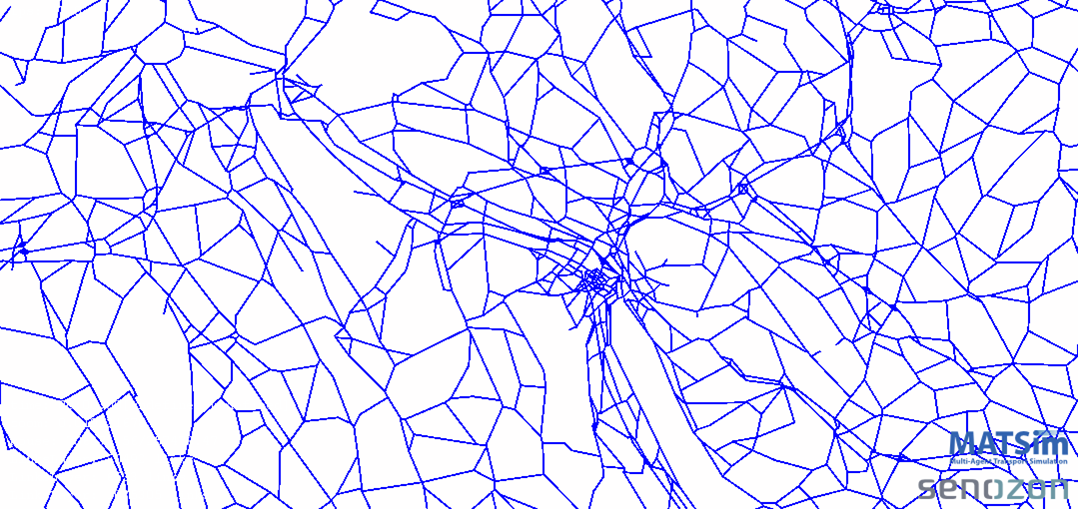
\includegraphics[width=0.8\textwidth,angle=0]{figures/planning.png}}%
  {\label{fig:planningnetwork}}%
  {}%
  \createsubfigure%
  {Navigation Network}%
	{
\includegraphics[width=0.8\textwidth,angle=0]{figures/navigation.png}}%
  {\label{fig:navigationnetwork}}%
  {}%
}%
{}

% ===============================================================================================
\subsection{Calibration, Verification, Validation and Policy Evaluation}
Calibration is a necessary task of any simulation study. Main calibration component is the utility function; it needs to reflect the preferences of the study area's population. A second prominent calibration screw is used for sample scenarios. To reduce the computational effort, initial explorative simulation runs are often performed as sample runs. In this case either the flow and storage capacity values of the mobility simulation or the network capacities need to be adapted accordingly.

Verification and validation, however, are of more concern for the microsimulation developer as detailed in Chapter \ref{ch:cvv}. Given a valuable estimate for demand and supply including a properly estimated utility function, from customer's perspective the simulation can be expected to generate valuable single run results out of the box.

The customer's responsibility is asked, at another place, though. Microsimulations are basically a sampling tool, just as a survey (see Section \ref{sec:variability}). A single run represents the sampling unit, the individual in surveys. This obviously means that microsimulation results must not to be presented as single runs but with the help of the usual statistical tools, e.g., by parameters with the common measures of spread or confidence intervals. That basically means that the customer is responsible to specify the sample size, the number of simulation runs feed with different random seeds. 

Policy evaluations are often based on count data, usually widely available and also showing substantial temporal variability. For MATSim, the count data need to be converted to represent the simulated average working day period.
 
% ===============================================================================================
In the modeling process as depicted in Section \ref{sec:alittletheory_modeling}, calibration, verification and validation are crucial steps. 

\emph{Calibration} is the process of adjusting model parameters to increase consistency of model outputs and observed target values \citep[][p.348]{HollanderLiu_Transportation_2007} \citep[see also][]{TrucanoEtAl_RESS_2006}. \citet[][Table 1]{HollanderLiu_Transportation_2007} list numerous studies that each calibrate a specific transport microsimulation. Further examples are \citet[][]{SmithEtAl_JTE_2008, KimEtAl_TRR_2005, RutterEtAl_JASA_2009}, microsimulation calibration guidelines are provided by \citet[][]{MilamChao_TRBATPM_2001, WegmannEverett_TechRep_CTRUT_2008, DowlingEtAl_manual_2002}. \citet[][Table 2]{HollanderLiu_Transportation_2007} describe measures of goodness-of-fit, that are productive for calibration. Due to the usually large number of model parameters, an automated process is favorable as far as possible. Essentially this is an optimization process \citep[][p.353]{HollanderLiu_Transportation_2007}, for which various established procedures exist \citep[e.g.,][p.41ff]{ZhangMa_ResRep_PATH_2008}. For MATSim, an automatic procedure adapting the plans to road counts was developed by \citet[][]{FloetteroedEtAl_TechRep_TRANSPOR_2008}. It is unclear however, if a certain loss of behavioral soundness is caused by adapting plans according to statistical matching. On the other hand, it is unclear anyway, to date, if the MATSim relaxation transitions should be given a behavioral meaning.

Verification is the procedure to test if a ``\emph{product is consistent with its specifications [...]}'' \citet[][p.330]{Petty_SokolowskiBanks_2010}. In verification, a perfect match can be achieved comparing the conceptual and the executable model (see Figure \ref{fig:modeling}) in contrast to validation, where the model is always an approximation to reality \citep[][p.145]{Kleijnen_EJOR_1995}. According to \citet[][p.331]{Petty_SokolowskiBanks_2010}, ``\emph{validation is the process of determining the degree to which the model is an accurate representation of the simuland.}'' Validation is difficult to standardize due to the variety of models and model purposes. Some measures, tests, and applications relevant to transport modeling are given by \citet[][Table 2]{MilamChao_TRBATPM_2001}, \citet[][]{Lima_TechRep_LMPO_2006}, \citet[][p.155]{KurthEtAl_TRBTDF_2006}, \citet[][p.157]{PendyalaBhat_TRBTDF_2006}, \citet[][p.8]{WegmannEverett_TechRep_CTRUT_2008}, \citet[][]{MilamChao_TRBATPM_2001, RoordaEtAl_TransResA_2008, HawasHameed_TPT_2009, SadekEtAl_TRR_2003, GouliasKitamura_TRR_1992}, \citet[][p.25]{CambridgeSystematics_manual_2008}, \citet[][p.145]{Kleijnen_EJOR_1995} (see also \citet[][]{David_EACSSS_2009}, \citet[][p.56]{SbaytiRoden_ResRep_AASHTO_2010}, \citet[][]{SchifferRossi_TRB_2009}). While for the 4-step procedure some validation standards have emerged \citep[e.g.,][]{BartonAschmanCambridgeSystematics_manual_1997}, a lack of standardization exists for activity-based models. \citet[][]{PendyalaBhat_TRBTDF_2006} say that ``\emph{despite the appeal of these models,}'' [activity- and tour-based travel demand modeling systems] \emph{``their widespread implementation appears to be hindered by the absence of a detailed validation and assessment of this new wave of model systems. Many MPOs will not adopt such models until they are tested.}'' \citet[][]{KurthEtAl_TRBTDF_2006} cites a statement made by Chandra Bhat and Frank Koppelman in a DRCOG e-mail discussion: ``\emph{Researchers and practitioners have not thought carefully enough about the criteria for validation of models. Researchers have the habit of asking practitioners to believe that activity- based methods will produce better impact assessment and forecasts because such models more appropriately represent the actual decision process (we plead guilty to this charge). There is a good basis for this line of thought, but researchers need to go beyond this argument. They need to develop clear validation criteria and demonstrate the value of activity-based methods in ways that are easily understood.}''

Often neglected, but important, is performing sensitivity analysis (sometimes dubbed ``what-if analysis'' \citep[][p.155]{Kleijnen_EJOR_1995}) \citep[][]{KurthEtAl_TRBTDF_2006, CambridgeSystematics_manual_2008, CFD_TRB_2007}. Sensitivity analysis is similar to assessing elasticity of a variable \citep[][p.3f]{WegmannEverett_TechRep_CTRUT_2008} and it tests reaction of the model to changed parameters including model input. This includes both testing the range of parameters for a given point in time, and analysis of the system's fore- and backcasting abilities \citep[e.g.,][p.56]{CFD_TRB_2007}, \citep[][]{CambridgeSystematics_manual_2008}. As forecasting is a vital objective of most transport models, this test is crucial. \citet[][p.158]{PendyalaBhat_TRBTDF_2006} puts it succinctly: ``\emph{There is no doubt that any model can be adjusted, refined, tweaked, and---if all else fails---hammered to replicate base-year conditions.}'' and concludes that ``\emph{the quality of a travel demand model system is better judged on its ability to respond to a range of scenarios and policies of interest.}'' In MATSim, a natural and interesting sensitivity test would be to compare the MATSim forecasts with the current actual state of Zurich network after addition of the bypass ``Westumfahrung'' in 2009 \citep[][]{BalmerEtAl_ResRep_bdktzrh_2009, Westumfahrung_Webpage_2008}.

As mentioned above, models are in general flexible enough to be calibrated to target data. Thus, validation \emph{must} be performed using a different data set than for preceding modeling steps \citep[][p.1]{CambridgeSystematics_manual_2008}, \citep[][p.56]{CFD_TRB_2007}, \citep[][p.18]{OrtuzarWillumsen_2001}. In statistics, this is called cross-validation. It is particularly important for forecasting models, which need to be general enough to capture temporal changes. Calibration and validation should thus be strictly separated, however, in microsimulation practice, according to the author's opinion, they are (too) often mixed, sometimes due to the vast amount of data required for model implementation and calibration. In MATSim, for example, after model calibration only road count data is left for validation \citep[][]{HorniEtAl_STRC_2009}; an example for a MATSim link volumes comparison between simulated and counted values is shown in Figure \ref{fig:countcomparison}. New data sources, such as road speed analyses based on GPS \citep[][]{HackneyEtAl_JGS_2007}, should be included.

Having said that, validation of a large-scale transport simulation is very difficult. Many central and comfortable characteristics of systems known from natural sciences are only seldom available for the social science, such as path-independence, decomposability, isolation, and on top of that repeatability of experiments. As a result, there is still a debate if social science actually can provide something similar as laws. \citet[][p.107ff]{Abel_1976} lists and discusses the 12 claims of the ``\emph{Verstehen Position}''; although, he finds contrary arguments to every claim, nevertheless, something definitely remains true, making social science model validation exceptionally difficult. For microsimulation results interpretation and model validation, it helped me to visualize the following example. A microsimulation forecast (or backcast) regarding the construction of the ``Westumfahrung Z�rich'' provides a probability distribution of scenarios, and it is essentially an exercise in Monte Carlo sampling. 4 years later we have exactly one actual state, and there is no way to assess the forecasted (or backcasted) probability distribution beyond checking that this actual state is contained in the probability distribution, and hopefully with high probability. There is nothing like Monte Carlo sampling when it comes to aggregate real system states. In other words the existing state is \emph{unique}. In essence, we thus compare an observed Dirac impulse with a computed probability distribution, which is a difficult undertaking.

% ----------
\createfigure%
{Example for a Link Volumes Comparison Between Simulation and Road Count Values}%
{Example for a Link Volumes Comparison Between Simulation and Road Count Values}%
{\label{fig:countcomparison}}%
{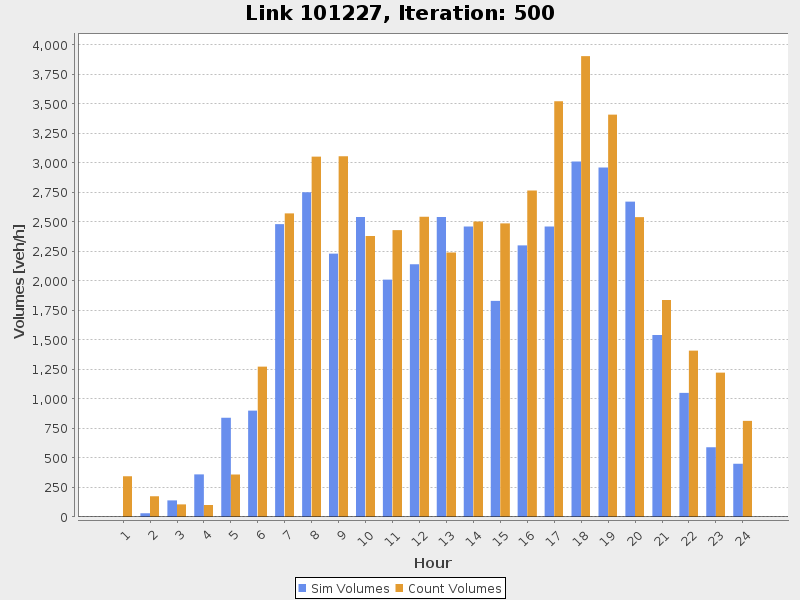
\includegraphics[width=0.8\textwidth, angle=0]{figures/link101227.png}}%
{}
% ----------

\ah{Noch mehr auf MATSim calibration, verification and validation eingehen.}

% ===============================================================================================
\subsection{Typical Output Data}
\label{sec:outputdata}

% ##################################################################################################################